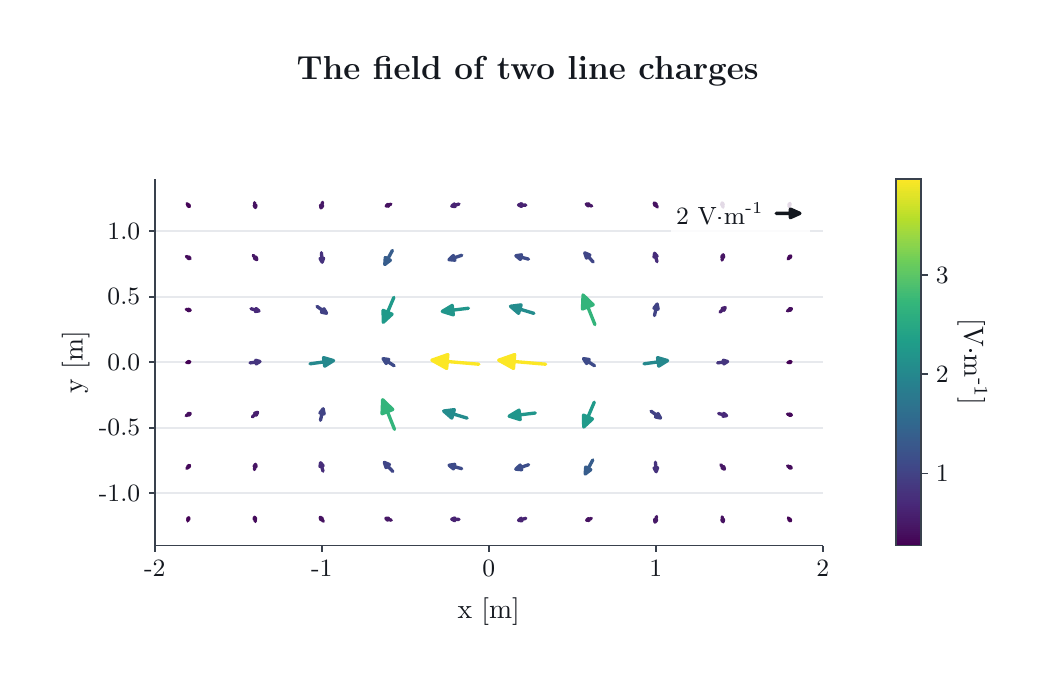
\begin{tikzpicture}[every node/.style={inner sep=0bp,outer sep=0bp}]
  \definecolor{qcA}{rgb}{1,1,1}
  \definecolor{qcB}{rgb}{0.078431,0.094118,0.121569}
  \definecolor{qcC}{rgb}{0.905882,0.913725,0.929412}
  \definecolor{qcD}{rgb}{0.267148,0.007009,0.331815}
  \definecolor{qcE}{rgb}{0.272384,0.047772,0.360886}
  \definecolor{qcF}{rgb}{0.275309,0.072066,0.380496}
  \definecolor{qcG}{rgb}{0.277762,0.09321,0.400283}
  \definecolor{qcH}{rgb}{0.281463,0.135381,0.44543}
  \definecolor{qcI}{rgb}{0.281711,0.139794,0.450499}
  \definecolor{qcJ}{rgb}{0.2783,0.098192,0.405257}
  \definecolor{qcK}{rgb}{0.269004,0.019894,0.341459}
  \definecolor{qcL}{rgb}{0.27075,0.03365,0.351149}
  \definecolor{qcM}{rgb}{0.276596,0.082916,0.390368}
  \definecolor{qcN}{rgb}{0.279489,0.177769,0.480108}
  \definecolor{qcO}{rgb}{0.250617,0.275339,0.529324}
  \definecolor{qcP}{rgb}{0.242484,0.29282,0.537725}
  \definecolor{qcQ}{rgb}{0.239054,0.305615,0.54}
  \definecolor{qcR}{rgb}{0.217409,0.363855,0.549948}
  \definecolor{qcS}{rgb}{0.275913,0.197462,0.489493}
  \definecolor{qcT}{rgb}{0.273905,0.06046,0.370669}
  \definecolor{qcU}{rgb}{0.280867,0.126428,0.435325}
  \definecolor{qcV}{rgb}{0.256465,0.262052,0.5223}
  \definecolor{qcW}{rgb}{0.198411,0.706786,0.482685}
  \definecolor{qcX}{rgb}{0.14092,0.547437,0.551417}
  \definecolor{qcY}{rgb}{0.130242,0.589866,0.54372}
  \definecolor{qcZ}{rgb}{0.125886,0.605274,0.540485}
  \definecolor{qcAA}{rgb}{0.258266,0.257591,0.519959}
  \definecolor{qcAB}{rgb}{0.281678,0.162414,0.473067}
  \definecolor{qcAC}{rgb}{0.272703,0.21178,0.496528}
  \definecolor{qcAD}{rgb}{0.14439,0.531974,0.553805}
  \definecolor{qcAE}{rgb}{0.987432,0.905348,0.14564}
  \definecolor{qcAF}{rgb}{0.223529,0.254902,0.301961}
  \definecolor{qcAG}{rgb}{0.267364,0.00843,0.332909}
  \definecolor{qcAH}{rgb}{0.268716,0.017786,0.339922}
  \definecolor{qcAI}{rgb}{0.27001,0.027601,0.346959}
  \definecolor{qcAJ}{rgb}{0.271245,0.037885,0.354021}
  \definecolor{qcAK}{rgb}{0.27242,0.048076,0.361108}
  \definecolor{qcAL}{rgb}{0.273535,0.057406,0.368219}
  \definecolor{qcAM}{rgb}{0.27459,0.06611,0.375354}
  \definecolor{qcAN}{rgb}{0.275582,0.074339,0.382512}
  \definecolor{qcAO}{rgb}{0.276512,0.082196,0.389693}
  \definecolor{qcAP}{rgb}{0.277378,0.089754,0.396898}
  \definecolor{qcAQ}{rgb}{0.278181,0.097068,0.404126}
  \definecolor{qcAR}{rgb}{0.278918,0.104178,0.411377}
  \definecolor{qcAS}{rgb}{0.279589,0.111116,0.41865}
  \definecolor{qcAT}{rgb}{0.280193,0.117907,0.425945}
  \definecolor{qcAU}{rgb}{0.280728,0.124573,0.433263}
  \definecolor{qcAV}{rgb}{0.281195,0.13113,0.440602}
  \definecolor{qcAW}{rgb}{0.281591,0.137592,0.447963}
  \definecolor{qcAX}{rgb}{0.281916,0.143971,0.455346}
  \definecolor{qcAY}{rgb}{0.282167,0.150277,0.46275}
  \definecolor{qcAZ}{rgb}{0.282345,0.156518,0.470175}
  \definecolor{qcBA}{rgb}{0.281465,0.164071,0.473814}
  \definecolor{qcBB}{rgb}{0.280434,0.171557,0.477228}
  \definecolor{qcBC}{rgb}{0.279307,0.17891,0.480642}
  \definecolor{qcBD}{rgb}{0.27808,0.186145,0.484055}
  \definecolor{qcBE}{rgb}{0.276752,0.193274,0.487467}
  \definecolor{qcBF}{rgb}{0.275318,0.20031,0.490878}
  \definecolor{qcBG}{rgb}{0.273776,0.207261,0.494289}
  \definecolor{qcBH}{rgb}{0.272122,0.214135,0.4977}
  \definecolor{qcBI}{rgb}{0.270352,0.22094,0.501109}
  \definecolor{qcBJ}{rgb}{0.268462,0.227683,0.504519}
  \definecolor{qcBK}{rgb}{0.266447,0.234368,0.507927}
  \definecolor{qcBL}{rgb}{0.264304,0.241002,0.511335}
  \definecolor{qcBM}{rgb}{0.262026,0.247588,0.514742}
  \definecolor{qcBN}{rgb}{0.259609,0.254131,0.518149}
  \definecolor{qcBO}{rgb}{0.257046,0.260635,0.521555}
  \definecolor{qcBP}{rgb}{0.25433,0.267102,0.524961}
  \definecolor{qcBQ}{rgb}{0.251455,0.273535,0.528366}
  \definecolor{qcBR}{rgb}{0.248413,0.279938,0.531771}
  \definecolor{qcBS}{rgb}{0.245195,0.286313,0.535175}
  \definecolor{qcBT}{rgb}{0.242533,0.292625,0.53769}
  \definecolor{qcBU}{rgb}{0.240919,0.298847,0.5388}
  \definecolor{qcBV}{rgb}{0.239218,0.305036,0.539898}
  \definecolor{qcBW}{rgb}{0.237427,0.311194,0.540984}
  \definecolor{qcBX}{rgb}{0.235541,0.317323,0.542059}
  \definecolor{qcBY}{rgb}{0.233559,0.323425,0.543121}
  \definecolor{qcBZ}{rgb}{0.231476,0.329503,0.544172}
  \definecolor{qcCA}{rgb}{0.229288,0.335557,0.54521}
  \definecolor{qcCB}{rgb}{0.226991,0.341589,0.546237}
  \definecolor{qcCC}{rgb}{0.22458,0.347601,0.547251}
  \definecolor{qcCD}{rgb}{0.22205,0.353594,0.548254}
  \definecolor{qcCE}{rgb}{0.219396,0.35957,0.549244}
  \definecolor{qcCF}{rgb}{0.216612,0.365529,0.550221}
  \definecolor{qcCG}{rgb}{0.213691,0.371473,0.551187}
  \definecolor{qcCH}{rgb}{0.210626,0.377402,0.552139}
  \definecolor{qcCI}{rgb}{0.207409,0.383318,0.55308}
  \definecolor{qcCJ}{rgb}{0.204031,0.389222,0.554008}
  \definecolor{qcCK}{rgb}{0.200483,0.395114,0.554923}
  \definecolor{qcCL}{rgb}{0.196753,0.400995,0.555826}
  \definecolor{qcCM}{rgb}{0.19283,0.406866,0.556716}
  \definecolor{qcCN}{rgb}{0.190883,0.412238,0.556986}
  \definecolor{qcCO}{rgb}{0.189301,0.417505,0.55712}
  \definecolor{qcCP}{rgb}{0.187662,0.422762,0.557239}
  \definecolor{qcCQ}{rgb}{0.185962,0.428012,0.557342}
  \definecolor{qcCR}{rgb}{0.184199,0.433253,0.55743}
  \definecolor{qcCS}{rgb}{0.182371,0.438488,0.557502}
  \definecolor{qcCT}{rgb}{0.180476,0.443716,0.557559}
  \definecolor{qcCU}{rgb}{0.17851,0.448938,0.5576}
  \definecolor{qcCV}{rgb}{0.176472,0.454154,0.557626}
  \definecolor{qcCW}{rgb}{0.174358,0.459365,0.557635}
  \definecolor{qcCX}{rgb}{0.172164,0.46457,0.557628}
  \definecolor{qcCY}{rgb}{0.169888,0.469771,0.557604}
  \definecolor{qcCZ}{rgb}{0.167525,0.474967,0.557565}
  \definecolor{qcDA}{rgb}{0.165071,0.480159,0.557509}
  \definecolor{qcDB}{rgb}{0.162521,0.485348,0.557436}
  \definecolor{qcDC}{rgb}{0.15987,0.490532,0.557346}
  \definecolor{qcDD}{rgb}{0.157114,0.495714,0.55724}
  \definecolor{qcDE}{rgb}{0.154245,0.500892,0.557116}
  \definecolor{qcDF}{rgb}{0.151256,0.506068,0.556975}
  \definecolor{qcDG}{rgb}{0.148705,0.511372,0.55666}
  \definecolor{qcDH}{rgb}{0.147557,0.517012,0.555915}
  \definecolor{qcDI}{rgb}{0.146385,0.522648,0.555143}
  \definecolor{qcDJ}{rgb}{0.145189,0.52828,0.554344}
  \definecolor{qcDK}{rgb}{0.143967,0.533908,0.553518}
  \definecolor{qcDL}{rgb}{0.14272,0.539533,0.552664}
  \definecolor{qcDM}{rgb}{0.141446,0.545154,0.551783}
  \definecolor{qcDN}{rgb}{0.140144,0.550772,0.550873}
  \definecolor{qcDO}{rgb}{0.138814,0.556388,0.549935}
  \definecolor{qcDP}{rgb}{0.137456,0.562002,0.548968}
  \definecolor{qcDQ}{rgb}{0.136067,0.567613,0.547971}
  \definecolor{qcDR}{rgb}{0.134648,0.573222,0.546945}
  \definecolor{qcDS}{rgb}{0.133196,0.57883,0.545889}
  \definecolor{qcDT}{rgb}{0.131712,0.584436,0.544802}
  \definecolor{qcDU}{rgb}{0.130194,0.590041,0.543684}
  \definecolor{qcDV}{rgb}{0.128641,0.595645,0.542535}
  \definecolor{qcDW}{rgb}{0.127051,0.601247,0.541354}
  \definecolor{qcDX}{rgb}{0.125424,0.606849,0.540141}
  \definecolor{qcDY}{rgb}{0.123758,0.612451,0.538895}
  \definecolor{qcDZ}{rgb}{0.12205,0.618052,0.537616}
  \definecolor{qcEA}{rgb}{0.124852,0.623254,0.535309}
  \definecolor{qcEB}{rgb}{0.12938,0.628298,0.532574}
  \definecolor{qcEC}{rgb}{0.133887,0.633338,0.529791}
  \definecolor{qcED}{rgb}{0.138375,0.638373,0.526958}
  \definecolor{qcEE}{rgb}{0.142846,0.643404,0.524076}
  \definecolor{qcEF}{rgb}{0.147302,0.648431,0.521142}
  \definecolor{qcEG}{rgb}{0.151743,0.653454,0.518155}
  \definecolor{qcEH}{rgb}{0.156171,0.658473,0.515115}
  \definecolor{qcEI}{rgb}{0.160586,0.663489,0.512019}
  \definecolor{qcEJ}{rgb}{0.16499,0.668502,0.508866}
  \definecolor{qcEK}{rgb}{0.169383,0.673511,0.505656}
  \definecolor{qcEL}{rgb}{0.173767,0.678518,0.502386}
  \definecolor{qcEM}{rgb}{0.178141,0.683521,0.499054}
  \definecolor{qcEN}{rgb}{0.182508,0.688522,0.49566}
  \definecolor{qcEO}{rgb}{0.186866,0.693521,0.492201}
  \definecolor{qcEP}{rgb}{0.191218,0.698516,0.488675}
  \definecolor{qcEQ}{rgb}{0.195563,0.70351,0.485081}
  \definecolor{qcER}{rgb}{0.199902,0.708501,0.481417}
  \definecolor{qcES}{rgb}{0.204236,0.713491,0.477681}
  \definecolor{qcET}{rgb}{0.210347,0.718428,0.473659}
  \definecolor{qcEU}{rgb}{0.224921,0.723111,0.468486}
  \definecolor{qcEV}{rgb}{0.238824,0.727785,0.463198}
  \definecolor{qcEW}{rgb}{0.252166,0.732451,0.457787}
  \definecolor{qcEX}{rgb}{0.265032,0.737108,0.452251}
  \definecolor{qcEY}{rgb}{0.277488,0.741757,0.446582}
  \definecolor{qcEZ}{rgb}{0.289589,0.746398,0.440774}
  \definecolor{qcFA}{rgb}{0.301378,0.751031,0.434821}
  \definecolor{qcFB}{rgb}{0.312892,0.755657,0.428715}
  \definecolor{qcFC}{rgb}{0.32416,0.760275,0.422448}
  \definecolor{qcFD}{rgb}{0.335208,0.764886,0.416012}
  \definecolor{qcFE}{rgb}{0.346059,0.76949,0.409397}
  \definecolor{qcFF}{rgb}{0.356731,0.774086,0.402592}
  \definecolor{qcFG}{rgb}{0.367241,0.778676,0.395587}
  \definecolor{qcFH}{rgb}{0.377603,0.783259,0.388368}
  \definecolor{qcFI}{rgb}{0.38783,0.787835,0.380921}
  \definecolor{qcFJ}{rgb}{0.397932,0.792404,0.373231}
  \definecolor{qcFK}{rgb}{0.407921,0.796967,0.365278}
  \definecolor{qcFL}{rgb}{0.417805,0.801524,0.357045}
  \definecolor{qcFM}{rgb}{0.427591,0.806075,0.348506}
  \definecolor{qcFN}{rgb}{0.441505,0.809891,0.341549}
  \definecolor{qcFO}{rgb}{0.457753,0.813229,0.33559}
  \definecolor{qcFP}{rgb}{0.473628,0.816552,0.32943}
  \definecolor{qcFQ}{rgb}{0.489169,0.81986,0.323056}
  \definecolor{qcFR}{rgb}{0.504411,0.823153,0.316454}
  \definecolor{qcFS}{rgb}{0.519383,0.826431,0.309607}
  \definecolor{qcFT}{rgb}{0.53411,0.829694,0.302496}
  \definecolor{qcFU}{rgb}{0.548613,0.832942,0.295099}
  \definecolor{qcFV}{rgb}{0.562912,0.836175,0.287392}
  \definecolor{qcFW}{rgb}{0.577024,0.839393,0.279346}
  \definecolor{qcFX}{rgb}{0.590964,0.842596,0.270928}
  \definecolor{qcFY}{rgb}{0.604745,0.845784,0.262097}
  \definecolor{qcFZ}{rgb}{0.61838,0.848958,0.252808}
  \definecolor{qcGA}{rgb}{0.63188,0.852116,0.243004}
  \definecolor{qcGB}{rgb}{0.645253,0.85526,0.232614}
  \definecolor{qcGC}{rgb}{0.65851,0.858389,0.221552}
  \definecolor{qcGD}{rgb}{0.671657,0.861503,0.209708}
  \definecolor{qcGE}{rgb}{0.684703,0.864603,0.196935}
  \definecolor{qcGF}{rgb}{0.697654,0.867688,0.183036}
  \definecolor{qcGG}{rgb}{0.710665,0.870702,0.168578}
  \definecolor{qcGH}{rgb}{0.726072,0.872742,0.16768}
  \definecolor{qcGI}{rgb}{0.74133,0.874757,0.166753}
  \definecolor{qcGJ}{rgb}{0.756449,0.876747,0.165798}
  \definecolor{qcGK}{rgb}{0.771439,0.878711,0.164812}
  \definecolor{qcGL}{rgb}{0.786307,0.880651,0.163797}
  \definecolor{qcGM}{rgb}{0.801063,0.882565,0.16275}
  \definecolor{qcGN}{rgb}{0.815713,0.884453,0.161671}
  \definecolor{qcGO}{rgb}{0.830265,0.886317,0.160559}
  \definecolor{qcGP}{rgb}{0.844723,0.888154,0.159414}
  \definecolor{qcGQ}{rgb}{0.859095,0.889967,0.158234}
  \definecolor{qcGR}{rgb}{0.873385,0.891753,0.157019}
  \definecolor{qcGS}{rgb}{0.887598,0.893513,0.155767}
  \definecolor{qcGT}{rgb}{0.901739,0.895248,0.154478}
  \definecolor{qcGU}{rgb}{0.915812,0.896956,0.15315}
  \definecolor{qcGV}{rgb}{0.929821,0.898638,0.151782}
  \definecolor{qcGW}{rgb}{0.943769,0.900294,0.150373}
  \definecolor{qcGX}{rgb}{0.95766,0.901924,0.148922}
  \definecolor{qcGY}{rgb}{0.971496,0.903527,0.147426}
  \definecolor{qcGZ}{rgb}{0.985282,0.905104,0.145885}
  \useasboundingbox (0bp,0bp) rectangle (360bp,225bp);
  % marey-key: figure
  \path[fill=qcA] (0bp,0bp) -- (360bp,0bp) -- (360bp,225bp) -- (0bp,225bp) -- cycle;
  % marey-role: annotation -- The field of two line charges
  \node[anchor=north,text=qcB,font=\bfseries\fontsize{13}{15.6}\selectfont] at (180bp,214.5bp) {The field of two line charges};
  % marey-key: figure/panel-0-0
  % marey-role: other:panel -- panel
  % marey-data: row = 0
  % marey-data: col = 0
  % marey-data: layers = 1
  % marey-data: x-tick-rule = all
  % marey-data: y-tick-rule = all
  % marey-role: decoration -- gridlines
  % marey-data: lines = 5
  \path[draw=qcC,line width=0.75bp] (45.757bp,57.43bp) -- (286.246bp,57.43bp) (45.757bp,81bp) -- (286.246bp,81bp) (45.757bp,104.569bp) -- (286.246bp,104.569bp) (45.757bp,128.138bp) -- (286.246bp,128.138bp) (45.757bp,151.707bp) -- (286.246bp,151.707bp);
  \begin{scope}
    \clip (45.757bp,38.575bp) -- (286.246bp,38.575bp) -- (286.246bp,170.563bp) -- (45.757bp,170.563bp) -- cycle;
    % marey-key: figure/panel-0-0/layer-0
    % marey-role: series -- series
    % marey-data: series =
    % marey-data: points = 70
    \path[fill=qcD,draw=qcD,line width=1.2bp,line cap=round,line join=round] (57.605bp,47.421bp) -- (57.817bp,48.119bp) (57.958bp,48.585bp) -- (57.607bp,48.183bp) -- (58.026bp,48.056bp) -- cycle (57.213bp,104.434bp) -- (57.895bp,104.596bp) (58.35bp,104.703bp) -- (57.847bp,104.8bp) -- (57.944bp,104.391bp) -- cycle (273.652bp,104.434bp) -- (274.335bp,104.596bp) (274.79bp,104.703bp) -- (274.286bp,104.8bp) -- (274.383bp,104.391bp) -- cycle (274.045bp,160.553bp) -- (274.256bp,161.251bp) (274.397bp,161.717bp) -- (274.047bp,161.315bp) -- (274.466bp,161.188bp) -- cycle;
    \path[fill=qcE,draw=qcE,line width=1.2bp,line cap=round,line join=round] (81.98bp,47.231bp) -- (81.8bp,48.157bp) (81.68bp,48.774bp) -- (81.523bp,48.103bp) -- (82.078bp,48.211bp) -- cycle (273.544bp,67.233bp) -- (274.356bp,66.783bp) (274.898bp,66.483bp) -- (274.491bp,67.027bp) -- (274.221bp,66.539bp) -- cycle (57.105bp,142.654bp) -- (57.917bp,142.204bp) (58.458bp,141.904bp) -- (58.052bp,142.448bp) -- (57.782bp,141.961bp) -- cycle (250.322bp,160.363bp) -- (250.142bp,161.289bp) (250.022bp,161.906bp) -- (249.865bp,161.235bp) -- (250.42bp,161.343bp) -- cycle;
    \path[fill=qcF,draw=qcF,line width=1.2bp,line cap=round,line join=round] (106.438bp,47.286bp) -- (105.767bp,48.146bp) (105.321bp,48.719bp) -- (105.51bp,47.945bp) -- (106.025bp,48.347bp) -- cycle (202.912bp,48.345bp) -- (201.907bp,47.934bp) (201.237bp,47.66bp) -- (202.03bp,47.633bp) -- (201.784bp,48.236bp) -- cycle (250.006bp,48.88bp) -- (250.206bp,47.827bp) (250.339bp,47.125bp) -- (250.521bp,47.887bp) -- (249.89bp,47.767bp) -- cycle (81.664bp,162.012bp) -- (81.864bp,160.959bp) (81.997bp,160.257bp) -- (82.179bp,161.019bp) -- (81.548bp,160.899bp) -- cycle (130.766bp,161.477bp) -- (129.76bp,161.066bp) (129.09bp,160.793bp) -- (129.884bp,160.765bp) -- (129.637bp,161.368bp) -- cycle (226.682bp,160.418bp) -- (226.012bp,161.278bp) (225.565bp,161.851bp) -- (225.754bp,161.077bp) -- (226.27bp,161.479bp) -- cycle;
    \path[fill=qcG,draw=qcG,line width=1.2bp,line cap=round,line join=round] (130.909bp,47.666bp) -- (129.732bp,48.07bp) (128.947bp,48.34bp) -- (129.61bp,47.717bp) -- (129.853bp,48.423bp) -- cycle (249.516bp,67.639bp) -- (250.304bp,66.702bp) (250.829bp,66.077bp) -- (250.585bp,66.938bp) -- (250.022bp,66.465bp) -- cycle (81.174bp,143.06bp) -- (81.962bp,142.123bp) (82.487bp,141.499bp) -- (82.243bp,142.36bp) -- (81.68bp,141.887bp) -- cycle (203.056bp,160.798bp) -- (201.878bp,161.202bp) (201.093bp,161.472bp) -- (201.757bp,160.849bp) -- (202bp,161.556bp) -- cycle;
    \path[fill=qcH,draw=qcH,line width=1.2bp,line cap=round,line join=round] (155.287bp,47.967bp) -- (153.715bp,48.01bp) (152.667bp,48.038bp) -- (153.702bp,47.538bp) -- (153.728bp,48.481bp) -- cycle (179.335bp,161.099bp) -- (177.764bp,161.142bp) (176.716bp,161.17bp) -- (177.751bp,160.67bp) -- (177.776bp,161.613bp) -- cycle;
    \path[fill=qcI,draw=qcI,line width=1.2bp,line cap=round,line join=round] (179.324bp,48.374bp) -- (177.766bp,47.928bp) (176.727bp,47.632bp) -- (177.9bp,47.461bp) -- (177.632bp,48.396bp) -- cycle (155.275bp,161.506bp) -- (153.717bp,161.061bp) (152.678bp,160.764bp) -- (153.851bp,160.593bp) -- (153.584bp,161.528bp) -- cycle;
    \path[fill=qcJ,draw=qcJ,line width=1.2bp,line cap=round,line join=round] (226.414bp,49.011bp) -- (226.065bp,47.801bp) (225.833bp,46.994bp) -- (226.428bp,47.696bp) -- (225.702bp,47.905bp) -- cycle (106.17bp,162.144bp) -- (105.821bp,160.933bp) (105.589bp,160.126bp) -- (106.184bp,160.829bp) -- (105.458bp,161.038bp) -- cycle;
    \path[fill=qcK,draw=qcK,line width=1.2bp,line cap=round,line join=round] (273.81bp,48.535bp) -- (274.303bp,47.896bp) (274.632bp,47.471bp) -- (274.495bp,48.044bp) -- (274.112bp,47.748bp) -- cycle (57.37bp,161.667bp) -- (57.864bp,161.028bp) (58.193bp,160.603bp) -- (58.055bp,161.176bp) -- (57.672bp,160.88bp) -- cycle;
    \path[fill=qcL,draw=qcL,line width=1.2bp,line cap=round,line join=round] (57.3bp,66.322bp) -- (57.878bp,66.965bp) (58.263bp,67.394bp) -- (57.685bp,67.138bp) -- (58.071bp,66.792bp) -- cycle (273.512bp,85.879bp) -- (274.363bp,85.68bp) (274.93bp,85.547bp) -- (274.423bp,85.935bp) -- (274.303bp,85.425bp) -- cycle (57.073bp,123.59bp) -- (57.923bp,123.391bp) (58.49bp,123.258bp) -- (57.983bp,123.646bp) -- (57.863bp,123.136bp) -- cycle (273.74bp,141.744bp) -- (274.317bp,142.387bp) (274.702bp,142.815bp) -- (274.124bp,142.56bp) -- (274.51bp,142.213bp) -- cycle;
    \path[fill=qcM,draw=qcM,line width=1.2bp,line cap=round,line join=round] (81.621bp,65.905bp) -- (81.872bp,67.049bp) (82.039bp,67.811bp) -- (81.529bp,67.124bp) -- (82.215bp,66.973bp) -- cycle (249.963bp,141.326bp) -- (250.214bp,142.47bp) (250.381bp,143.233bp) -- (249.871bp,142.545bp) -- (250.557bp,142.395bp) -- cycle;
    \path[fill=qcN,draw=qcN,line width=1.2bp,line cap=round,line join=round] (106.319bp,65.34bp) -- (105.791bp,67.162bp) (105.44bp,68.376bp) -- (105.245bp,67.003bp) -- (106.338bp,67.32bp) -- cycle (226.563bp,140.762bp) -- (226.035bp,142.583bp) (225.684bp,143.797bp) -- (225.489bp,142.425bp) -- (226.582bp,142.741bp) -- cycle;
    \path[fill=qcO,draw=qcO,line width=1.2bp,line cap=round,line join=round] (131.46bp,65.211bp) -- (129.622bp,67.188bp) (128.396bp,68.506bp) -- (129.028bp,66.636bp) -- (130.215bp,67.739bp) -- cycle (203.607bp,140.632bp) -- (201.768bp,142.609bp) (200.542bp,143.927bp) -- (201.175bp,142.057bp) -- (202.361bp,143.161bp) -- cycle;
    \path[fill=qcP,draw=qcP,line width=1.2bp,line cap=round,line join=round] (156.254bp,66.241bp) -- (153.521bp,66.981bp) (151.699bp,67.475bp) -- (153.299bp,66.161bp) -- (153.743bp,67.801bp) -- cycle (131.923bp,103.293bp) -- (129.529bp,104.824bp) (127.933bp,105.844bp) -- (129.07bp,104.106bp) -- (129.988bp,105.542bp) -- cycle (204.07bp,103.293bp) -- (201.676bp,104.824bp) (200.079bp,105.844bp) -- (201.216bp,104.106bp) -- (202.135bp,105.542bp) -- cycle (180.303bp,141.663bp) -- (177.57bp,142.403bp) (175.748bp,142.896bp) -- (177.348bp,141.583bp) -- (177.792bp,143.223bp) -- cycle;
    \path[fill=qcQ,draw=qcQ,line width=1.2bp,line cap=round,line join=round] (180.338bp,67.657bp) -- (177.563bp,66.698bp) (175.713bp,66.059bp) -- (177.851bp,65.866bp) -- (177.276bp,67.531bp) -- cycle (156.289bp,143.078bp) -- (153.514bp,142.12bp) (151.665bp,141.481bp) -- (153.802bp,141.287bp) -- (153.227bp,142.952bp) -- cycle;
    \path[fill=qcR,draw=qcR,line width=1.2bp,line cap=round,line join=round] (203.446bp,69.386bp) -- (201.8bp,66.352bp) (200.703bp,64.33bp) -- (202.71bp,65.859bp) -- (200.89bp,66.846bp) -- cycle (131.3bp,144.807bp) -- (129.654bp,141.774bp) (128.556bp,139.752bp) -- (130.564bp,141.28bp) -- (128.744bp,142.268bp) -- cycle;
    \path[fill=qcS,draw=qcS,line width=1.2bp,line cap=round,line join=round] (225.994bp,68.575bp) -- (226.149bp,66.515bp) (226.252bp,65.141bp) -- (226.767bp,66.561bp) -- (225.531bp,66.468bp) -- cycle (105.75bp,143.996bp) -- (105.905bp,141.936bp) (106.008bp,140.563bp) -- (106.523bp,141.983bp) -- (105.287bp,141.89bp) -- cycle;
    \path[fill=qcT,draw=qcT,line width=1.2bp,line cap=round,line join=round] (57.054bp,85.31bp) -- (57.927bp,85.794bp) (58.509bp,86.116bp) -- (57.782bp,86.056bp) -- (58.072bp,85.532bp) -- cycle (273.493bp,123.021bp) -- (274.367bp,123.505bp) (274.949bp,123.827bp) -- (274.222bp,123.767bp) -- (274.512bp,123.243bp) -- cycle;
    \path[fill=qcU,draw=qcU,line width=1.2bp,line cap=round,line join=round] (80.891bp,84.901bp) -- (82.018bp,85.876bp) (82.769bp,86.526bp) -- (81.726bp,86.214bp) -- (82.311bp,85.538bp) -- cycle (249.233bp,122.612bp) -- (250.36bp,123.587bp) (251.111bp,124.237bp) -- (250.067bp,123.925bp) -- (250.653bp,123.249bp) -- cycle;
    \path[fill=qcV,draw=qcV,line width=1.2bp,line cap=round,line join=round] (105.396bp,83.638bp) -- (105.976bp,86.128bp) (106.362bp,87.789bp) -- (105.229bp,86.302bp) -- (106.723bp,85.955bp) -- cycle (225.64bp,121.349bp) -- (226.22bp,123.839bp) (226.606bp,125.5bp) -- (225.473bp,124.013bp) -- (226.967bp,123.665bp) -- cycle;
    \path[fill=qcW,draw=qcW,line width=1.2bp,line cap=round,line join=round] (132.064bp,80.376bp) -- (129.501bp,86.781bp) (127.792bp,91.05bp) -- (127.579bp,86.012bp) -- (131.422bp,87.55bp) -- cycle (204.211bp,118.087bp) -- (201.647bp,124.491bp) (199.938bp,128.761bp) -- (199.726bp,123.723bp) -- (203.569bp,125.26bp) -- cycle;
    \path[fill=qcX,draw=qcX,line width=1.2bp,line cap=round,line join=round] (158.197bp,84.437bp) -- (153.133bp,85.969bp) (149.757bp,86.99bp) -- (152.673bp,84.449bp) -- (153.592bp,87.488bp) -- cycle (182.246bp,122.148bp) -- (177.182bp,123.679bp) (173.806bp,124.7bp) -- (176.722bp,122.16bp) -- (177.641bp,125.199bp) -- cycle;
    \path[fill=qcY,draw=qcY,line width=1.2bp,line cap=round,line join=round] (182.732bp,86.28bp) -- (177.084bp,85.6bp) (173.32bp,85.147bp) -- (177.288bp,83.906bp) -- (176.881bp,87.294bp) -- cycle (158.683bp,123.991bp) -- (153.036bp,123.311bp) (149.271bp,122.858bp) -- (153.24bp,121.617bp) -- (152.832bp,125.005bp) -- cycle;
    \path[fill=qcZ,draw=qcZ,line width=1.2bp,line cap=round,line join=round] (203.974bp,90.185bp) -- (201.695bp,84.819bp) (200.175bp,81.242bp) -- (203.304bp,84.135bp) -- (200.085bp,85.503bp) -- cycle (131.827bp,127.895bp) -- (129.548bp,122.53bp) (128.029bp,118.953bp) -- (131.158bp,121.846bp) -- (127.939bp,123.214bp) -- cycle;
    \path[fill=qcAA,draw=qcAA,line width=1.2bp,line cap=round,line join=round] (224.402bp,86.947bp) -- (226.468bp,85.467bp) (227.845bp,84.48bp) -- (226.912bp,86.086bp) -- (226.024bp,84.847bp) -- cycle (104.158bp,124.658bp) -- (106.223bp,123.177bp) (107.601bp,122.191bp) -- (106.667bp,123.797bp) -- (105.779bp,122.558bp) -- cycle;
    \path[fill=qcAB,draw=qcAB,line width=1.2bp,line cap=round,line join=round] (248.738bp,86.11bp) -- (250.459bp,85.634bp) (251.607bp,85.316bp) -- (250.602bp,86.15bp) -- (250.316bp,85.118bp) -- cycle (80.396bp,123.821bp) -- (82.117bp,123.345bp) (83.265bp,123.027bp) -- (82.26bp,123.861bp) -- (81.974bp,122.828bp) -- cycle;
    \path[fill=qcAC,draw=qcAC,line width=1.2bp,line cap=round,line join=round] (80.038bp,104.32bp) -- (82.189bp,104.619bp) (83.623bp,104.818bp) -- (82.099bp,105.264bp) -- (82.278bp,103.973bp) -- cycle (248.38bp,104.32bp) -- (250.531bp,104.619bp) (251.965bp,104.818bp) -- (250.441bp,105.264bp) -- (250.62bp,103.973bp) -- cycle;
    \path[fill=qcAD,draw=qcAD,line width=1.2bp,line cap=round,line join=round] (101.64bp,103.986bp) -- (106.727bp,104.685bp) (110.118bp,105.151bp) -- (106.517bp,106.211bp) -- (106.937bp,103.159bp) -- cycle (221.884bp,103.986bp) -- (226.971bp,104.685bp) (230.363bp,105.151bp) -- (226.762bp,106.211bp) -- (227.181bp,103.159bp) -- cycle;
    \path[fill=qcAE,draw=qcAE,line width=1.2bp,line cap=round,line join=round] (162.431bp,103.842bp) -- (151.053bp,104.82bp) (145.523bp,105.296bp) -- (150.839bp,102.332bp) -- (151.267bp,107.308bp) -- cycle (186.479bp,103.842bp) -- (175.102bp,104.82bp) (169.572bp,105.296bp) -- (174.888bp,102.332bp) -- (175.316bp,107.308bp) -- cycle;
    % marey-role: legend -- quiver key
    \path[fill=qcA,fill opacity=0.85] (231.7bp,150.238bp) -- (281.746bp,150.238bp) -- (281.746bp,166.063bp) -- (231.7bp,166.063bp) -- cycle;
    \path[fill=qcB,draw=qcB,line width=1.2bp,line cap=round,line join=round] (269.452bp,158.15bp) -- (274.578bp,158.15bp) (277.996bp,158.15bp) -- (274.578bp,159.688bp) -- (274.578bp,156.612bp) -- cycle;
    \node[anchor=east,text=qcB,font=\fontsize{9}{10.8}\selectfont] at (264.952bp,158.15bp) {2 V\textperiodcentered{}m\textsuperscript{-1}};
  \end{scope}
  % marey-role: axis -- x [m]
  % marey-data: side = bottom
  % marey-data: unit = m
  % marey-data: prefix =
  % marey-data: ticks = 5
  % marey-data: tick-rule = all
  \path[draw=qcAF,line width=0.675bp] (45.757bp,38.575bp) -- (286.246bp,38.575bp);
  \path[draw=qcAF,line width=0.675bp] (45.757bp,38.575bp) -- (45.757bp,36.325bp) (105.879bp,38.575bp) -- (105.879bp,36.325bp) (166.001bp,38.575bp) -- (166.001bp,36.325bp) (226.123bp,38.575bp) -- (226.123bp,36.325bp) (286.246bp,38.575bp) -- (286.246bp,36.325bp);
  \node[anchor=north,text=qcB,font=\fontsize{9}{10.8}\selectfont] at (45.757bp,33.325bp) {-2};
  \node[anchor=north,text=qcB,font=\fontsize{9}{10.8}\selectfont] at (105.879bp,33.325bp) {-1};
  \node[anchor=north,text=qcB,font=\fontsize{9}{10.8}\selectfont] at (166.001bp,33.325bp) {0};
  \node[anchor=north,text=qcB,font=\fontsize{9}{10.8}\selectfont] at (226.123bp,33.325bp) {1};
  \node[anchor=north,text=qcB,font=\fontsize{9}{10.8}\selectfont] at (286.246bp,33.325bp) {2};
  \node[anchor=north,text=qcB,font=\fontsize{10}{12}\selectfont] at (166.001bp,19.75bp) {x [m]};
  % marey-role: axis -- y [m]
  % marey-data: side = left
  % marey-data: unit = m
  % marey-data: prefix =
  % marey-data: ticks = 5
  % marey-data: tick-rule = all
  \path[draw=qcAF,line width=0.675bp] (45.757bp,38.575bp) -- (45.757bp,170.563bp);
  \path[draw=qcAF,line width=0.675bp] (45.757bp,57.43bp) -- (43.507bp,57.43bp) (45.757bp,81bp) -- (43.507bp,81bp) (45.757bp,104.569bp) -- (43.507bp,104.569bp) (45.757bp,128.138bp) -- (43.507bp,128.138bp) (45.757bp,151.707bp) -- (43.507bp,151.707bp);
  \node[anchor=east,text=qcB,font=\fontsize{9}{10.8}\selectfont] at (40.507bp,57.43bp) {-1.0};
  \node[anchor=east,text=qcB,font=\fontsize{9}{10.8}\selectfont] at (40.507bp,81bp) {-0.5};
  \node[anchor=east,text=qcB,font=\fontsize{9}{10.8}\selectfont] at (40.507bp,104.569bp) {0.0};
  \node[anchor=east,text=qcB,font=\fontsize{9}{10.8}\selectfont] at (40.507bp,128.138bp) {0.5};
  \node[anchor=east,text=qcB,font=\fontsize{9}{10.8}\selectfont] at (40.507bp,151.707bp) {1.0};
  \node[anchor=base,text=qcB,rotate=90,font=\fontsize{10}{12}\selectfont] at (19.75bp,104.569bp) {y [m]};
  % marey-role: other:colorbar -- [V·m⁻¹]
  % marey-data: title = [V·m⁻¹]
  % marey-data: unit = V·m⁻¹
  % marey-data: steps = 176
  \path[fill=qcAG] (312.746bp,38.575bp) -- (321.746bp,38.575bp) -- (321.746bp,39.587bp) -- (312.746bp,39.587bp) -- cycle;
  \path[fill=qcAH] (312.746bp,39.325bp) -- (321.746bp,39.325bp) -- (321.746bp,40.337bp) -- (312.746bp,40.337bp) -- cycle;
  \path[fill=qcAI] (312.746bp,40.075bp) -- (321.746bp,40.075bp) -- (321.746bp,41.087bp) -- (312.746bp,41.087bp) -- cycle;
  \path[fill=qcAJ] (312.746bp,40.825bp) -- (321.746bp,40.825bp) -- (321.746bp,41.837bp) -- (312.746bp,41.837bp) -- cycle;
  \path[fill=qcAK] (312.746bp,41.575bp) -- (321.746bp,41.575bp) -- (321.746bp,42.587bp) -- (312.746bp,42.587bp) -- cycle;
  \path[fill=qcAL] (312.746bp,42.325bp) -- (321.746bp,42.325bp) -- (321.746bp,43.337bp) -- (312.746bp,43.337bp) -- cycle;
  \path[fill=qcAM] (312.746bp,43.075bp) -- (321.746bp,43.075bp) -- (321.746bp,44.087bp) -- (312.746bp,44.087bp) -- cycle;
  \path[fill=qcAN] (312.746bp,43.825bp) -- (321.746bp,43.825bp) -- (321.746bp,44.837bp) -- (312.746bp,44.837bp) -- cycle;
  \path[fill=qcAO] (312.746bp,44.574bp) -- (321.746bp,44.574bp) -- (321.746bp,45.587bp) -- (312.746bp,45.587bp) -- cycle;
  \path[fill=qcAP] (312.746bp,45.324bp) -- (321.746bp,45.324bp) -- (321.746bp,46.337bp) -- (312.746bp,46.337bp) -- cycle;
  \path[fill=qcAQ] (312.746bp,46.074bp) -- (321.746bp,46.074bp) -- (321.746bp,47.087bp) -- (312.746bp,47.087bp) -- cycle;
  \path[fill=qcAR] (312.746bp,46.824bp) -- (321.746bp,46.824bp) -- (321.746bp,47.837bp) -- (312.746bp,47.837bp) -- cycle;
  \path[fill=qcAS] (312.746bp,47.574bp) -- (321.746bp,47.574bp) -- (321.746bp,48.587bp) -- (312.746bp,48.587bp) -- cycle;
  \path[fill=qcAT] (312.746bp,48.324bp) -- (321.746bp,48.324bp) -- (321.746bp,49.336bp) -- (312.746bp,49.336bp) -- cycle;
  \path[fill=qcAU] (312.746bp,49.074bp) -- (321.746bp,49.074bp) -- (321.746bp,50.086bp) -- (312.746bp,50.086bp) -- cycle;
  \path[fill=qcAV] (312.746bp,49.824bp) -- (321.746bp,49.824bp) -- (321.746bp,50.836bp) -- (312.746bp,50.836bp) -- cycle;
  \path[fill=qcAW] (312.746bp,50.574bp) -- (321.746bp,50.574bp) -- (321.746bp,51.586bp) -- (312.746bp,51.586bp) -- cycle;
  \path[fill=qcAX] (312.746bp,51.324bp) -- (321.746bp,51.324bp) -- (321.746bp,52.336bp) -- (312.746bp,52.336bp) -- cycle;
  \path[fill=qcAY] (312.746bp,52.074bp) -- (321.746bp,52.074bp) -- (321.746bp,53.086bp) -- (312.746bp,53.086bp) -- cycle;
  \path[fill=qcAZ] (312.746bp,52.824bp) -- (321.746bp,52.824bp) -- (321.746bp,53.836bp) -- (312.746bp,53.836bp) -- cycle;
  \path[fill=qcBA] (312.746bp,53.574bp) -- (321.746bp,53.574bp) -- (321.746bp,54.586bp) -- (312.746bp,54.586bp) -- cycle;
  \path[fill=qcBB] (312.746bp,54.324bp) -- (321.746bp,54.324bp) -- (321.746bp,55.336bp) -- (312.746bp,55.336bp) -- cycle;
  \path[fill=qcBC] (312.746bp,55.073bp) -- (321.746bp,55.073bp) -- (321.746bp,56.086bp) -- (312.746bp,56.086bp) -- cycle;
  \path[fill=qcBD] (312.746bp,55.823bp) -- (321.746bp,55.823bp) -- (321.746bp,56.836bp) -- (312.746bp,56.836bp) -- cycle;
  \path[fill=qcBE] (312.746bp,56.573bp) -- (321.746bp,56.573bp) -- (321.746bp,57.586bp) -- (312.746bp,57.586bp) -- cycle;
  \path[fill=qcBF] (312.746bp,57.323bp) -- (321.746bp,57.323bp) -- (321.746bp,58.336bp) -- (312.746bp,58.336bp) -- cycle;
  \path[fill=qcBG] (312.746bp,58.073bp) -- (321.746bp,58.073bp) -- (321.746bp,59.086bp) -- (312.746bp,59.086bp) -- cycle;
  \path[fill=qcBH] (312.746bp,58.823bp) -- (321.746bp,58.823bp) -- (321.746bp,59.835bp) -- (312.746bp,59.835bp) -- cycle;
  \path[fill=qcBI] (312.746bp,59.573bp) -- (321.746bp,59.573bp) -- (321.746bp,60.585bp) -- (312.746bp,60.585bp) -- cycle;
  \path[fill=qcBJ] (312.746bp,60.323bp) -- (321.746bp,60.323bp) -- (321.746bp,61.335bp) -- (312.746bp,61.335bp) -- cycle;
  \path[fill=qcBK] (312.746bp,61.073bp) -- (321.746bp,61.073bp) -- (321.746bp,62.085bp) -- (312.746bp,62.085bp) -- cycle;
  \path[fill=qcBL] (312.746bp,61.823bp) -- (321.746bp,61.823bp) -- (321.746bp,62.835bp) -- (312.746bp,62.835bp) -- cycle;
  \path[fill=qcBM] (312.746bp,62.573bp) -- (321.746bp,62.573bp) -- (321.746bp,63.585bp) -- (312.746bp,63.585bp) -- cycle;
  \path[fill=qcBN] (312.746bp,63.323bp) -- (321.746bp,63.323bp) -- (321.746bp,64.335bp) -- (312.746bp,64.335bp) -- cycle;
  \path[fill=qcBO] (312.746bp,64.073bp) -- (321.746bp,64.073bp) -- (321.746bp,65.085bp) -- (312.746bp,65.085bp) -- cycle;
  \path[fill=qcBP] (312.746bp,64.823bp) -- (321.746bp,64.823bp) -- (321.746bp,65.835bp) -- (312.746bp,65.835bp) -- cycle;
  \path[fill=qcBQ] (312.746bp,65.572bp) -- (321.746bp,65.572bp) -- (321.746bp,66.585bp) -- (312.746bp,66.585bp) -- cycle;
  \path[fill=qcBR] (312.746bp,66.322bp) -- (321.746bp,66.322bp) -- (321.746bp,67.335bp) -- (312.746bp,67.335bp) -- cycle;
  \path[fill=qcBS] (312.746bp,67.072bp) -- (321.746bp,67.072bp) -- (321.746bp,68.085bp) -- (312.746bp,68.085bp) -- cycle;
  \path[fill=qcBT] (312.746bp,67.822bp) -- (321.746bp,67.822bp) -- (321.746bp,68.835bp) -- (312.746bp,68.835bp) -- cycle;
  \path[fill=qcBU] (312.746bp,68.572bp) -- (321.746bp,68.572bp) -- (321.746bp,69.585bp) -- (312.746bp,69.585bp) -- cycle;
  \path[fill=qcBV] (312.746bp,69.322bp) -- (321.746bp,69.322bp) -- (321.746bp,70.334bp) -- (312.746bp,70.334bp) -- cycle;
  \path[fill=qcBW] (312.746bp,70.072bp) -- (321.746bp,70.072bp) -- (321.746bp,71.084bp) -- (312.746bp,71.084bp) -- cycle;
  \path[fill=qcBX] (312.746bp,70.822bp) -- (321.746bp,70.822bp) -- (321.746bp,71.834bp) -- (312.746bp,71.834bp) -- cycle;
  \path[fill=qcBY] (312.746bp,71.572bp) -- (321.746bp,71.572bp) -- (321.746bp,72.584bp) -- (312.746bp,72.584bp) -- cycle;
  \path[fill=qcBZ] (312.746bp,72.322bp) -- (321.746bp,72.322bp) -- (321.746bp,73.334bp) -- (312.746bp,73.334bp) -- cycle;
  \path[fill=qcCA] (312.746bp,73.072bp) -- (321.746bp,73.072bp) -- (321.746bp,74.084bp) -- (312.746bp,74.084bp) -- cycle;
  \path[fill=qcCB] (312.746bp,73.822bp) -- (321.746bp,73.822bp) -- (321.746bp,74.834bp) -- (312.746bp,74.834bp) -- cycle;
  \path[fill=qcCC] (312.746bp,74.572bp) -- (321.746bp,74.572bp) -- (321.746bp,75.584bp) -- (312.746bp,75.584bp) -- cycle;
  \path[fill=qcCD] (312.746bp,75.322bp) -- (321.746bp,75.322bp) -- (321.746bp,76.334bp) -- (312.746bp,76.334bp) -- cycle;
  \path[fill=qcCE] (312.746bp,76.071bp) -- (321.746bp,76.071bp) -- (321.746bp,77.084bp) -- (312.746bp,77.084bp) -- cycle;
  \path[fill=qcCF] (312.746bp,76.821bp) -- (321.746bp,76.821bp) -- (321.746bp,77.834bp) -- (312.746bp,77.834bp) -- cycle;
  \path[fill=qcCG] (312.746bp,77.571bp) -- (321.746bp,77.571bp) -- (321.746bp,78.584bp) -- (312.746bp,78.584bp) -- cycle;
  \path[fill=qcCH] (312.746bp,78.321bp) -- (321.746bp,78.321bp) -- (321.746bp,79.334bp) -- (312.746bp,79.334bp) -- cycle;
  \path[fill=qcCI] (312.746bp,79.071bp) -- (321.746bp,79.071bp) -- (321.746bp,80.084bp) -- (312.746bp,80.084bp) -- cycle;
  \path[fill=qcCJ] (312.746bp,79.821bp) -- (321.746bp,79.821bp) -- (321.746bp,80.833bp) -- (312.746bp,80.833bp) -- cycle;
  \path[fill=qcCK] (312.746bp,80.571bp) -- (321.746bp,80.571bp) -- (321.746bp,81.583bp) -- (312.746bp,81.583bp) -- cycle;
  \path[fill=qcCL] (312.746bp,81.321bp) -- (321.746bp,81.321bp) -- (321.746bp,82.333bp) -- (312.746bp,82.333bp) -- cycle;
  \path[fill=qcCM] (312.746bp,82.071bp) -- (321.746bp,82.071bp) -- (321.746bp,83.083bp) -- (312.746bp,83.083bp) -- cycle;
  \path[fill=qcCN] (312.746bp,82.821bp) -- (321.746bp,82.821bp) -- (321.746bp,83.833bp) -- (312.746bp,83.833bp) -- cycle;
  \path[fill=qcCO] (312.746bp,83.571bp) -- (321.746bp,83.571bp) -- (321.746bp,84.583bp) -- (312.746bp,84.583bp) -- cycle;
  \path[fill=qcCP] (312.746bp,84.321bp) -- (321.746bp,84.321bp) -- (321.746bp,85.333bp) -- (312.746bp,85.333bp) -- cycle;
  \path[fill=qcCQ] (312.746bp,85.071bp) -- (321.746bp,85.071bp) -- (321.746bp,86.083bp) -- (312.746bp,86.083bp) -- cycle;
  \path[fill=qcCR] (312.746bp,85.821bp) -- (321.746bp,85.821bp) -- (321.746bp,86.833bp) -- (312.746bp,86.833bp) -- cycle;
  \path[fill=qcCS] (312.746bp,86.57bp) -- (321.746bp,86.57bp) -- (321.746bp,87.583bp) -- (312.746bp,87.583bp) -- cycle;
  \path[fill=qcCT] (312.746bp,87.32bp) -- (321.746bp,87.32bp) -- (321.746bp,88.333bp) -- (312.746bp,88.333bp) -- cycle;
  \path[fill=qcCU] (312.746bp,88.07bp) -- (321.746bp,88.07bp) -- (321.746bp,89.083bp) -- (312.746bp,89.083bp) -- cycle;
  \path[fill=qcCV] (312.746bp,88.82bp) -- (321.746bp,88.82bp) -- (321.746bp,89.833bp) -- (312.746bp,89.833bp) -- cycle;
  \path[fill=qcCW] (312.746bp,89.57bp) -- (321.746bp,89.57bp) -- (321.746bp,90.583bp) -- (312.746bp,90.583bp) -- cycle;
  \path[fill=qcCX] (312.746bp,90.32bp) -- (321.746bp,90.32bp) -- (321.746bp,91.333bp) -- (312.746bp,91.333bp) -- cycle;
  \path[fill=qcCY] (312.746bp,91.07bp) -- (321.746bp,91.07bp) -- (321.746bp,92.082bp) -- (312.746bp,92.082bp) -- cycle;
  \path[fill=qcCZ] (312.746bp,91.82bp) -- (321.746bp,91.82bp) -- (321.746bp,92.832bp) -- (312.746bp,92.832bp) -- cycle;
  \path[fill=qcDA] (312.746bp,92.57bp) -- (321.746bp,92.57bp) -- (321.746bp,93.582bp) -- (312.746bp,93.582bp) -- cycle;
  \path[fill=qcDB] (312.746bp,93.32bp) -- (321.746bp,93.32bp) -- (321.746bp,94.332bp) -- (312.746bp,94.332bp) -- cycle;
  \path[fill=qcDC] (312.746bp,94.07bp) -- (321.746bp,94.07bp) -- (321.746bp,95.082bp) -- (312.746bp,95.082bp) -- cycle;
  \path[fill=qcDD] (312.746bp,94.82bp) -- (321.746bp,94.82bp) -- (321.746bp,95.832bp) -- (312.746bp,95.832bp) -- cycle;
  \path[fill=qcDE] (312.746bp,95.57bp) -- (321.746bp,95.57bp) -- (321.746bp,96.582bp) -- (312.746bp,96.582bp) -- cycle;
  \path[fill=qcDF] (312.746bp,96.32bp) -- (321.746bp,96.32bp) -- (321.746bp,97.332bp) -- (312.746bp,97.332bp) -- cycle;
  \path[fill=qcDG] (312.746bp,97.069bp) -- (321.746bp,97.069bp) -- (321.746bp,98.082bp) -- (312.746bp,98.082bp) -- cycle;
  \path[fill=qcDH] (312.746bp,97.819bp) -- (321.746bp,97.819bp) -- (321.746bp,98.832bp) -- (312.746bp,98.832bp) -- cycle;
  \path[fill=qcDI] (312.746bp,98.569bp) -- (321.746bp,98.569bp) -- (321.746bp,99.582bp) -- (312.746bp,99.582bp) -- cycle;
  \path[fill=qcDJ] (312.746bp,99.319bp) -- (321.746bp,99.319bp) -- (321.746bp,100.332bp) -- (312.746bp,100.332bp) -- cycle;
  \path[fill=qcDK] (312.746bp,100.069bp) -- (321.746bp,100.069bp) -- (321.746bp,101.082bp) -- (312.746bp,101.082bp) -- cycle;
  \path[fill=qcDL] (312.746bp,100.819bp) -- (321.746bp,100.819bp) -- (321.746bp,101.832bp) -- (312.746bp,101.832bp) -- cycle;
  \path[fill=qcDM] (312.746bp,101.569bp) -- (321.746bp,101.569bp) -- (321.746bp,102.581bp) -- (312.746bp,102.581bp) -- cycle;
  \path[fill=qcDN] (312.746bp,102.319bp) -- (321.746bp,102.319bp) -- (321.746bp,103.331bp) -- (312.746bp,103.331bp) -- cycle;
  \path[fill=qcDO] (312.746bp,103.069bp) -- (321.746bp,103.069bp) -- (321.746bp,104.081bp) -- (312.746bp,104.081bp) -- cycle;
  \path[fill=qcDP] (312.746bp,103.819bp) -- (321.746bp,103.819bp) -- (321.746bp,104.831bp) -- (312.746bp,104.831bp) -- cycle;
  \path[fill=qcDQ] (312.746bp,104.569bp) -- (321.746bp,104.569bp) -- (321.746bp,105.581bp) -- (312.746bp,105.581bp) -- cycle;
  \path[fill=qcDR] (312.746bp,105.319bp) -- (321.746bp,105.319bp) -- (321.746bp,106.331bp) -- (312.746bp,106.331bp) -- cycle;
  \path[fill=qcDS] (312.746bp,106.069bp) -- (321.746bp,106.069bp) -- (321.746bp,107.081bp) -- (312.746bp,107.081bp) -- cycle;
  \path[fill=qcDT] (312.746bp,106.819bp) -- (321.746bp,106.819bp) -- (321.746bp,107.831bp) -- (312.746bp,107.831bp) -- cycle;
  \path[fill=qcDU] (312.746bp,107.568bp) -- (321.746bp,107.568bp) -- (321.746bp,108.581bp) -- (312.746bp,108.581bp) -- cycle;
  \path[fill=qcDV] (312.746bp,108.318bp) -- (321.746bp,108.318bp) -- (321.746bp,109.331bp) -- (312.746bp,109.331bp) -- cycle;
  \path[fill=qcDW] (312.746bp,109.068bp) -- (321.746bp,109.068bp) -- (321.746bp,110.081bp) -- (312.746bp,110.081bp) -- cycle;
  \path[fill=qcDX] (312.746bp,109.818bp) -- (321.746bp,109.818bp) -- (321.746bp,110.831bp) -- (312.746bp,110.831bp) -- cycle;
  \path[fill=qcDY] (312.746bp,110.568bp) -- (321.746bp,110.568bp) -- (321.746bp,111.581bp) -- (312.746bp,111.581bp) -- cycle;
  \path[fill=qcDZ] (312.746bp,111.318bp) -- (321.746bp,111.318bp) -- (321.746bp,112.331bp) -- (312.746bp,112.331bp) -- cycle;
  \path[fill=qcEA] (312.746bp,112.068bp) -- (321.746bp,112.068bp) -- (321.746bp,113.08bp) -- (312.746bp,113.08bp) -- cycle;
  \path[fill=qcEB] (312.746bp,112.818bp) -- (321.746bp,112.818bp) -- (321.746bp,113.83bp) -- (312.746bp,113.83bp) -- cycle;
  \path[fill=qcEC] (312.746bp,113.568bp) -- (321.746bp,113.568bp) -- (321.746bp,114.58bp) -- (312.746bp,114.58bp) -- cycle;
  \path[fill=qcED] (312.746bp,114.318bp) -- (321.746bp,114.318bp) -- (321.746bp,115.33bp) -- (312.746bp,115.33bp) -- cycle;
  \path[fill=qcEE] (312.746bp,115.068bp) -- (321.746bp,115.068bp) -- (321.746bp,116.08bp) -- (312.746bp,116.08bp) -- cycle;
  \path[fill=qcEF] (312.746bp,115.818bp) -- (321.746bp,115.818bp) -- (321.746bp,116.83bp) -- (312.746bp,116.83bp) -- cycle;
  \path[fill=qcEG] (312.746bp,116.568bp) -- (321.746bp,116.568bp) -- (321.746bp,117.58bp) -- (312.746bp,117.58bp) -- cycle;
  \path[fill=qcEH] (312.746bp,117.318bp) -- (321.746bp,117.318bp) -- (321.746bp,118.33bp) -- (312.746bp,118.33bp) -- cycle;
  \path[fill=qcEI] (312.746bp,118.067bp) -- (321.746bp,118.067bp) -- (321.746bp,119.08bp) -- (312.746bp,119.08bp) -- cycle;
  \path[fill=qcEJ] (312.746bp,118.817bp) -- (321.746bp,118.817bp) -- (321.746bp,119.83bp) -- (312.746bp,119.83bp) -- cycle;
  \path[fill=qcEK] (312.746bp,119.567bp) -- (321.746bp,119.567bp) -- (321.746bp,120.58bp) -- (312.746bp,120.58bp) -- cycle;
  \path[fill=qcEL] (312.746bp,120.317bp) -- (321.746bp,120.317bp) -- (321.746bp,121.33bp) -- (312.746bp,121.33bp) -- cycle;
  \path[fill=qcEM] (312.746bp,121.067bp) -- (321.746bp,121.067bp) -- (321.746bp,122.08bp) -- (312.746bp,122.08bp) -- cycle;
  \path[fill=qcEN] (312.746bp,121.817bp) -- (321.746bp,121.817bp) -- (321.746bp,122.83bp) -- (312.746bp,122.83bp) -- cycle;
  \path[fill=qcEO] (312.746bp,122.567bp) -- (321.746bp,122.567bp) -- (321.746bp,123.579bp) -- (312.746bp,123.579bp) -- cycle;
  \path[fill=qcEP] (312.746bp,123.317bp) -- (321.746bp,123.317bp) -- (321.746bp,124.329bp) -- (312.746bp,124.329bp) -- cycle;
  \path[fill=qcEQ] (312.746bp,124.067bp) -- (321.746bp,124.067bp) -- (321.746bp,125.079bp) -- (312.746bp,125.079bp) -- cycle;
  \path[fill=qcER] (312.746bp,124.817bp) -- (321.746bp,124.817bp) -- (321.746bp,125.829bp) -- (312.746bp,125.829bp) -- cycle;
  \path[fill=qcES] (312.746bp,125.567bp) -- (321.746bp,125.567bp) -- (321.746bp,126.579bp) -- (312.746bp,126.579bp) -- cycle;
  \path[fill=qcET] (312.746bp,126.317bp) -- (321.746bp,126.317bp) -- (321.746bp,127.329bp) -- (312.746bp,127.329bp) -- cycle;
  \path[fill=qcEU] (312.746bp,127.067bp) -- (321.746bp,127.067bp) -- (321.746bp,128.079bp) -- (312.746bp,128.079bp) -- cycle;
  \path[fill=qcEV] (312.746bp,127.817bp) -- (321.746bp,127.817bp) -- (321.746bp,128.829bp) -- (312.746bp,128.829bp) -- cycle;
  \path[fill=qcEW] (312.746bp,128.566bp) -- (321.746bp,128.566bp) -- (321.746bp,129.579bp) -- (312.746bp,129.579bp) -- cycle;
  \path[fill=qcEX] (312.746bp,129.316bp) -- (321.746bp,129.316bp) -- (321.746bp,130.329bp) -- (312.746bp,130.329bp) -- cycle;
  \path[fill=qcEY] (312.746bp,130.066bp) -- (321.746bp,130.066bp) -- (321.746bp,131.079bp) -- (312.746bp,131.079bp) -- cycle;
  \path[fill=qcEZ] (312.746bp,130.816bp) -- (321.746bp,130.816bp) -- (321.746bp,131.829bp) -- (312.746bp,131.829bp) -- cycle;
  \path[fill=qcFA] (312.746bp,131.566bp) -- (321.746bp,131.566bp) -- (321.746bp,132.579bp) -- (312.746bp,132.579bp) -- cycle;
  \path[fill=qcFB] (312.746bp,132.316bp) -- (321.746bp,132.316bp) -- (321.746bp,133.329bp) -- (312.746bp,133.329bp) -- cycle;
  \path[fill=qcFC] (312.746bp,133.066bp) -- (321.746bp,133.066bp) -- (321.746bp,134.078bp) -- (312.746bp,134.078bp) -- cycle;
  \path[fill=qcFD] (312.746bp,133.816bp) -- (321.746bp,133.816bp) -- (321.746bp,134.828bp) -- (312.746bp,134.828bp) -- cycle;
  \path[fill=qcFE] (312.746bp,134.566bp) -- (321.746bp,134.566bp) -- (321.746bp,135.578bp) -- (312.746bp,135.578bp) -- cycle;
  \path[fill=qcFF] (312.746bp,135.316bp) -- (321.746bp,135.316bp) -- (321.746bp,136.328bp) -- (312.746bp,136.328bp) -- cycle;
  \path[fill=qcFG] (312.746bp,136.066bp) -- (321.746bp,136.066bp) -- (321.746bp,137.078bp) -- (312.746bp,137.078bp) -- cycle;
  \path[fill=qcFH] (312.746bp,136.816bp) -- (321.746bp,136.816bp) -- (321.746bp,137.828bp) -- (312.746bp,137.828bp) -- cycle;
  \path[fill=qcFI] (312.746bp,137.566bp) -- (321.746bp,137.566bp) -- (321.746bp,138.578bp) -- (312.746bp,138.578bp) -- cycle;
  \path[fill=qcFJ] (312.746bp,138.316bp) -- (321.746bp,138.316bp) -- (321.746bp,139.328bp) -- (312.746bp,139.328bp) -- cycle;
  \path[fill=qcFK] (312.746bp,139.065bp) -- (321.746bp,139.065bp) -- (321.746bp,140.078bp) -- (312.746bp,140.078bp) -- cycle;
  \path[fill=qcFL] (312.746bp,139.815bp) -- (321.746bp,139.815bp) -- (321.746bp,140.828bp) -- (312.746bp,140.828bp) -- cycle;
  \path[fill=qcFM] (312.746bp,140.565bp) -- (321.746bp,140.565bp) -- (321.746bp,141.578bp) -- (312.746bp,141.578bp) -- cycle;
  \path[fill=qcFN] (312.746bp,141.315bp) -- (321.746bp,141.315bp) -- (321.746bp,142.328bp) -- (312.746bp,142.328bp) -- cycle;
  \path[fill=qcFO] (312.746bp,142.065bp) -- (321.746bp,142.065bp) -- (321.746bp,143.078bp) -- (312.746bp,143.078bp) -- cycle;
  \path[fill=qcFP] (312.746bp,142.815bp) -- (321.746bp,142.815bp) -- (321.746bp,143.828bp) -- (312.746bp,143.828bp) -- cycle;
  \path[fill=qcFQ] (312.746bp,143.565bp) -- (321.746bp,143.565bp) -- (321.746bp,144.577bp) -- (312.746bp,144.577bp) -- cycle;
  \path[fill=qcFR] (312.746bp,144.315bp) -- (321.746bp,144.315bp) -- (321.746bp,145.327bp) -- (312.746bp,145.327bp) -- cycle;
  \path[fill=qcFS] (312.746bp,145.065bp) -- (321.746bp,145.065bp) -- (321.746bp,146.077bp) -- (312.746bp,146.077bp) -- cycle;
  \path[fill=qcFT] (312.746bp,145.815bp) -- (321.746bp,145.815bp) -- (321.746bp,146.827bp) -- (312.746bp,146.827bp) -- cycle;
  \path[fill=qcFU] (312.746bp,146.565bp) -- (321.746bp,146.565bp) -- (321.746bp,147.577bp) -- (312.746bp,147.577bp) -- cycle;
  \path[fill=qcFV] (312.746bp,147.315bp) -- (321.746bp,147.315bp) -- (321.746bp,148.327bp) -- (312.746bp,148.327bp) -- cycle;
  \path[fill=qcFW] (312.746bp,148.065bp) -- (321.746bp,148.065bp) -- (321.746bp,149.077bp) -- (312.746bp,149.077bp) -- cycle;
  \path[fill=qcFX] (312.746bp,148.815bp) -- (321.746bp,148.815bp) -- (321.746bp,149.827bp) -- (312.746bp,149.827bp) -- cycle;
  \path[fill=qcFY] (312.746bp,149.564bp) -- (321.746bp,149.564bp) -- (321.746bp,150.577bp) -- (312.746bp,150.577bp) -- cycle;
  \path[fill=qcFZ] (312.746bp,150.314bp) -- (321.746bp,150.314bp) -- (321.746bp,151.327bp) -- (312.746bp,151.327bp) -- cycle;
  \path[fill=qcGA] (312.746bp,151.064bp) -- (321.746bp,151.064bp) -- (321.746bp,152.077bp) -- (312.746bp,152.077bp) -- cycle;
  \path[fill=qcGB] (312.746bp,151.814bp) -- (321.746bp,151.814bp) -- (321.746bp,152.827bp) -- (312.746bp,152.827bp) -- cycle;
  \path[fill=qcGC] (312.746bp,152.564bp) -- (321.746bp,152.564bp) -- (321.746bp,153.577bp) -- (312.746bp,153.577bp) -- cycle;
  \path[fill=qcGD] (312.746bp,153.314bp) -- (321.746bp,153.314bp) -- (321.746bp,154.327bp) -- (312.746bp,154.327bp) -- cycle;
  \path[fill=qcGE] (312.746bp,154.064bp) -- (321.746bp,154.064bp) -- (321.746bp,155.076bp) -- (312.746bp,155.076bp) -- cycle;
  \path[fill=qcGF] (312.746bp,154.814bp) -- (321.746bp,154.814bp) -- (321.746bp,155.826bp) -- (312.746bp,155.826bp) -- cycle;
  \path[fill=qcGG] (312.746bp,155.564bp) -- (321.746bp,155.564bp) -- (321.746bp,156.576bp) -- (312.746bp,156.576bp) -- cycle;
  \path[fill=qcGH] (312.746bp,156.314bp) -- (321.746bp,156.314bp) -- (321.746bp,157.326bp) -- (312.746bp,157.326bp) -- cycle;
  \path[fill=qcGI] (312.746bp,157.064bp) -- (321.746bp,157.064bp) -- (321.746bp,158.076bp) -- (312.746bp,158.076bp) -- cycle;
  \path[fill=qcGJ] (312.746bp,157.814bp) -- (321.746bp,157.814bp) -- (321.746bp,158.826bp) -- (312.746bp,158.826bp) -- cycle;
  \path[fill=qcGK] (312.746bp,158.564bp) -- (321.746bp,158.564bp) -- (321.746bp,159.576bp) -- (312.746bp,159.576bp) -- cycle;
  \path[fill=qcGL] (312.746bp,159.314bp) -- (321.746bp,159.314bp) -- (321.746bp,160.326bp) -- (312.746bp,160.326bp) -- cycle;
  \path[fill=qcGM] (312.746bp,160.063bp) -- (321.746bp,160.063bp) -- (321.746bp,161.076bp) -- (312.746bp,161.076bp) -- cycle;
  \path[fill=qcGN] (312.746bp,160.813bp) -- (321.746bp,160.813bp) -- (321.746bp,161.826bp) -- (312.746bp,161.826bp) -- cycle;
  \path[fill=qcGO] (312.746bp,161.563bp) -- (321.746bp,161.563bp) -- (321.746bp,162.576bp) -- (312.746bp,162.576bp) -- cycle;
  \path[fill=qcGP] (312.746bp,162.313bp) -- (321.746bp,162.313bp) -- (321.746bp,163.326bp) -- (312.746bp,163.326bp) -- cycle;
  \path[fill=qcGQ] (312.746bp,163.063bp) -- (321.746bp,163.063bp) -- (321.746bp,164.076bp) -- (312.746bp,164.076bp) -- cycle;
  \path[fill=qcGR] (312.746bp,163.813bp) -- (321.746bp,163.813bp) -- (321.746bp,164.826bp) -- (312.746bp,164.826bp) -- cycle;
  \path[fill=qcGS] (312.746bp,164.563bp) -- (321.746bp,164.563bp) -- (321.746bp,165.575bp) -- (312.746bp,165.575bp) -- cycle;
  \path[fill=qcGT] (312.746bp,165.313bp) -- (321.746bp,165.313bp) -- (321.746bp,166.325bp) -- (312.746bp,166.325bp) -- cycle;
  \path[fill=qcGU] (312.746bp,166.063bp) -- (321.746bp,166.063bp) -- (321.746bp,167.075bp) -- (312.746bp,167.075bp) -- cycle;
  \path[fill=qcGV] (312.746bp,166.813bp) -- (321.746bp,166.813bp) -- (321.746bp,167.825bp) -- (312.746bp,167.825bp) -- cycle;
  \path[fill=qcGW] (312.746bp,167.563bp) -- (321.746bp,167.563bp) -- (321.746bp,168.575bp) -- (312.746bp,168.575bp) -- cycle;
  \path[fill=qcGX] (312.746bp,168.313bp) -- (321.746bp,168.313bp) -- (321.746bp,169.325bp) -- (312.746bp,169.325bp) -- cycle;
  \path[fill=qcGY] (312.746bp,169.063bp) -- (321.746bp,169.063bp) -- (321.746bp,170.075bp) -- (312.746bp,170.075bp) -- cycle;
  \path[fill=qcGZ] (312.746bp,169.813bp) -- (321.746bp,169.813bp) -- (321.746bp,170.563bp) -- (312.746bp,170.563bp) -- cycle;
  \path[draw=qcAF,line width=0.675bp] (312.746bp,38.575bp) -- (321.746bp,38.575bp) -- (321.746bp,170.563bp) -- (312.746bp,170.563bp) -- cycle;
  % marey-role: axis -- [V·m⁻¹]
  % marey-data: side = right
  % marey-data: unit = V·m⁻¹
  % marey-data: prefix =
  % marey-data: ticks = 3
  % marey-data: tick-rule = all
  \path[draw=qcAF,line width=0.675bp] (321.746bp,64.496bp) -- (323.996bp,64.496bp) (321.746bp,100.18bp) -- (323.996bp,100.18bp) (321.746bp,135.864bp) -- (323.996bp,135.864bp);
  \node[anchor=west,text=qcB,font=\fontsize{9}{10.8}\selectfont] at (326.996bp,64.496bp) {1};
  \node[anchor=west,text=qcB,font=\fontsize{9}{10.8}\selectfont] at (326.996bp,100.18bp) {2};
  \node[anchor=west,text=qcB,font=\fontsize{9}{10.8}\selectfont] at (326.996bp,135.864bp) {3};
  \node[anchor=base,text=qcB,rotate=-90,font=\fontsize{10}{12}\selectfont] at (337.25bp,104.569bp) {[V\textperiodcentered{}m\textsuperscript{-1}]};
\end{tikzpicture}
